\documentclass[oneside,a4paper,14pt]{extarticle}
\usepackage[a4paper,letterpaper,top=20mm,bottom=20mm,left=20mm,right=10mm]{geometry}
\usepackage[russian]{babel}
\usepackage{indentfirst}
\usepackage{graphicx}
\usepackage{caption}
\usepackage{titlesec}
\usepackage{minted, fancyvrb}
\usepackage{hyperref}
\usepackage{enumitem}

% Форматирование листингов с кодом
\setminted{style = rainbow_dash, fontsize = \small} % https://pygments.org/styles/

% Форматирование заголовков
\titleformat{\section}{\normalsize\bfseries}{\thesection}{1em}{}
\titleformat{\subsection}{\normalsize\bfseries}{\thesubsection}{1em}{}
\titleformat{\subsubsection}{\normalsize\bfseries}{\thesubsubsection}{1em}{}

% Интерлиньяж и абзац
\renewcommand\baselinestretch{1.33}

\setlength{\parindent}{1.25cm}  % длина красной строки

% Для всех списков
\setlist[enumerate]{
  left=\parindent,       % отступ слева
  label=\arabic*.,       % цифры
  itemsep=0pt,           % расстояние между пунктами
  topsep=5pt,            % отступ сверху
  partopsep=0pt,         % дополнительный отступ сверху, если абзац до списка
  parsep=0pt             % отступ между абзацами внутри пункта
}

\setlist[itemize]{
  left=\parindent,       % отступ слева
  itemsep=0pt,           % расстояние между пунктами
  topsep=5pt,            % отступ сверху
  partopsep=0pt,
  parsep=0pt
}

% Гиперссылки
\hypersetup{
  colorlinks=true,
  linkcolor=black,
  urlcolor=blue,
  pdfborder={0 0 0},
  pdftitle={Qt6 приложение для управления устройствами умного дома},
  pdfauthor={Черкасов А.А.}
}

\begin{document}

\newpage
\thispagestyle{empty}
\begin{center}
  МИНИСТЕРСТВО НАУКИ И ВЫСШЕГО ОБРАЗОВАНИЯ РОССИЙСКОЙ ФЕДЕРАЦИИ ФЕДЕРАЛЬНОЕ ГОСУДАРСТВЕННОЕ БЮДЖЕТНОЕ ОБРАЗОВАТЕЛЬНОЕ УЧРЕЖДЕНИЕ ВЫСШЕГО ОБРАЗОВАНИЯ\\
  «ВЯТСКИЙ ГОСУДАРСТВЕННЫЙ УНИВЕРСИТЕТ»\\
  Институт математики и информационных систем\\
  Факультет автоматики и вычислительной техники\\
  Кафедра электронных вычислительных машин
\end{center}
\vspace{10mm}

\hfill
\begin{tabular}{l}
  \footnotesize Дата сдачи на проверку:                                          \\
  \footnotesize <<\rule[-1mm]{5mm}{0.10mm}\/>>\rule[-1mm]{20mm}{0.10mm}\ 2025 г. \\
  \footnotesize Проверено:                                                       \\
  \footnotesize <<\rule[-1mm]{5mm}{0.10mm}\/>>\rule[-1mm]{20mm}{0.10mm}\ 2025 г. \\
\end{tabular}
\vfill

\begin{center}
  Связывание приложения на C++ с Qt6 с базой данных под управлением PostgreSQL.\\
  Отчёт по лабораторной работе №4\\
  по дисциплине\\
  <<Управление данными>>\\
\end{center}
\vspace{25mm}
\noindent
\begin{tabular}{ll}
  Разработал студент гр. ИВТб-2301-05-00 & \hspace{18mm}\rule[-1mm]{30mm}{0.10mm}\,/Черкасов А. А./ \\
                                         & \hspace{25.5mm}\footnotesize(подпись)                    \\
  Старший Преподователь                  & \hspace{18mm}\rule[-1mm]{30mm}{0.10mm}\,/Клюкин В. Л./   \\
                                         & \hspace{25.5mm}\footnotesize(подпись)                    \\
\end{tabular}

\noindent
\begin{tabular}{lp{58mm}r}
  Работа защищена &  & \hspace{13mm}<<\rule[-1mm]{5mm}{0.10mm}\/>>\rule[-1mm]{30mm}{0.10mm}\ 2025 г.
\end{tabular}
\vfill

\begin{center}
  Киров\\
  2025
\end{center}

\newpage\thispagestyle{plain}

\section*{Цели лабораторной работы}
\begin{itemize}
  \item[$-$] познакомиться с библиотекой libpqxx в языке C++ для связывания приложения с БД;
  \item[$-$] освоить на практике основы взаимодействия с БД под управлением PostgreSQL в приложении на C++ с Qt6.
\end{itemize}

\section*{Задание}
Создать приложение с графическим интерфейсом на языке С++, использующее БД, разработанную в предыдущих лабораторных работах, со следующими требованиями:
\begin{enumerate}
  \item Названия колонок, кнопок, объектов ввода/вывода на русском языке.
  \item Запрет ввода отрицательных значений.
  \item Ввод данных для выборки регистронезависимый (используются функции UPPER или LOWER).
  \item Для любой таблицы с внешним ключом реализовать:
        \begin{itemize}
          \item[$-$] вывод, удаление и изменение данных таблицы;
          \item[$-$] проверку ввода уже имеющихся данных с выводом сообщения пользователю;
          \item[$-$] удаление при подтверждении;
          \item[$-$] выполнение фильтра (выборки) по значениям строк.
        \end{itemize}
  \item При добавлении новой строки внешний ключ выбирается из списка значений родительской таблицы.
  \item Сохранение или удаление строки реализовано с помощью функции PL/pgSQL.
  \item Фильтрация значений при поиске производится через запрос, а не в полученной коллекции.
\end{enumerate}

\clearpage
\section*{Реализация приложения}

\subsection*{Диаграмма классов}
\begin{figure}[H]
  \centering
  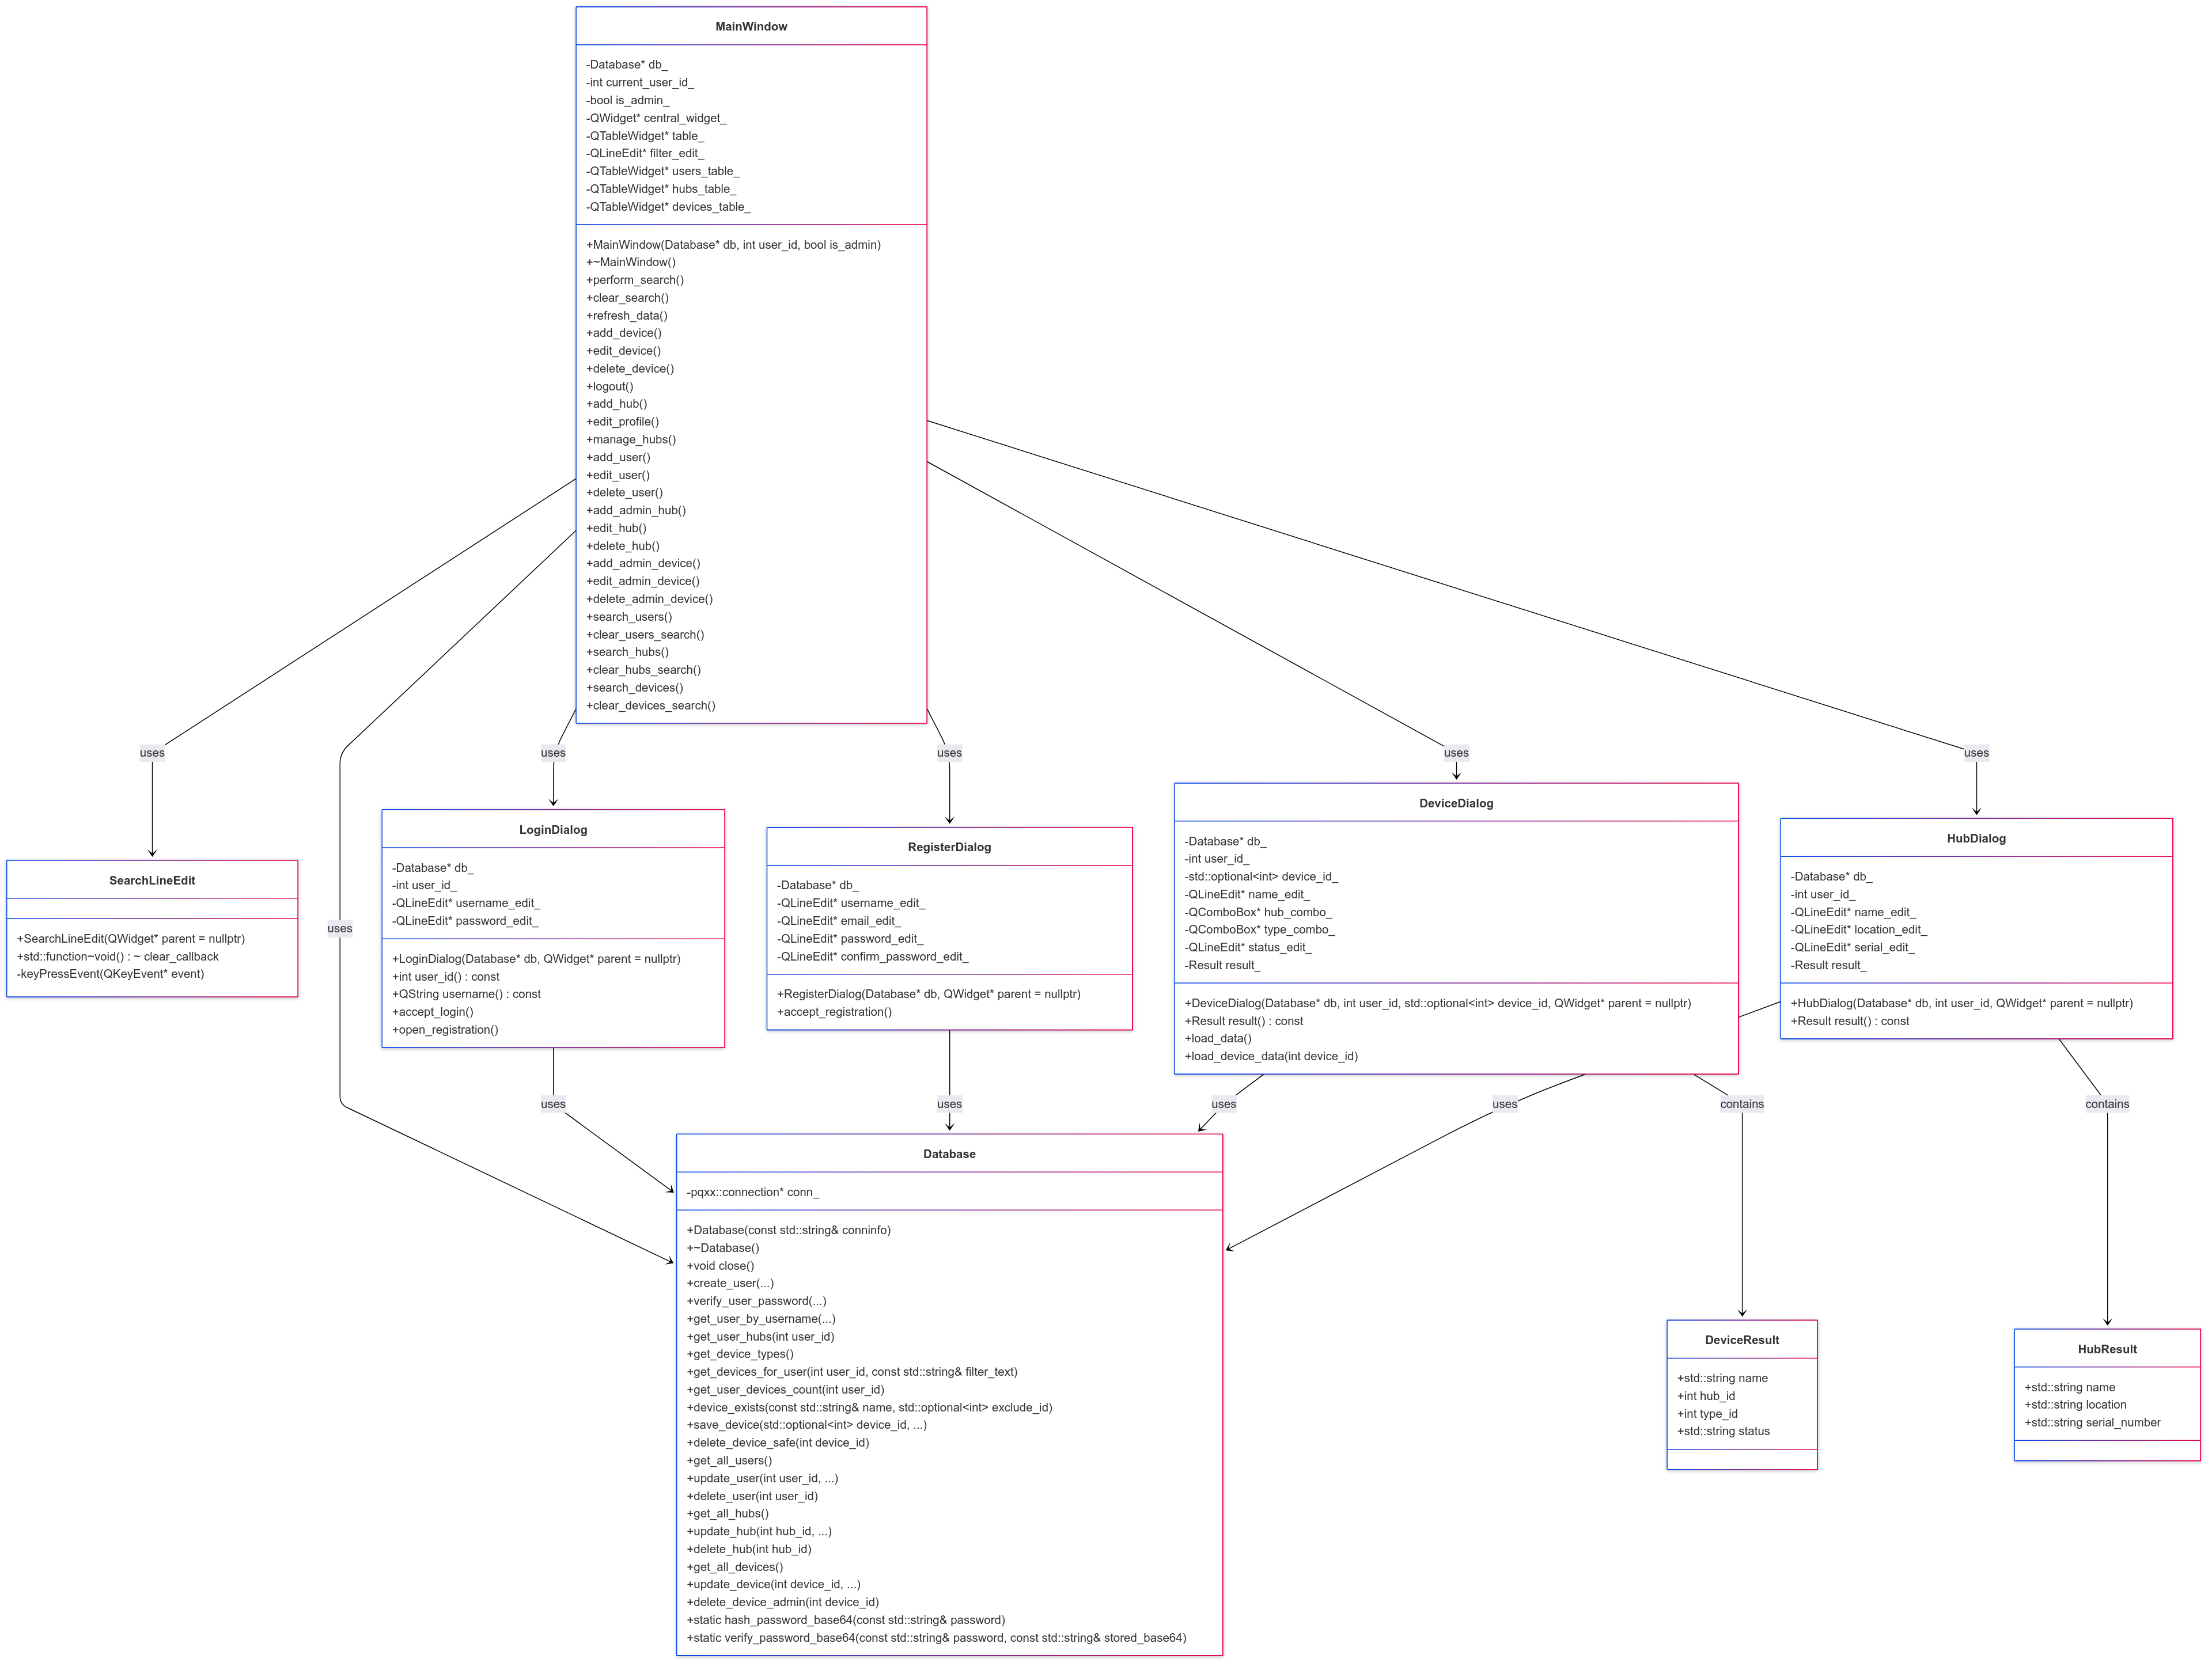
\includegraphics[width=0.95\textwidth]{pics/class_diagram.png}
  \caption{Диаграмма классов приложения}
\end{figure}

Диаграмма классов показывает архитектуру приложения и организацию работы с базой данных:
\begin{itemize}
  \item[$-$] \texttt{Database} $-$ класс для подключения и выполнения операций с PostgreSQL через libpqxx
  \item[$-$] \texttt{MainWindow} $-$ главное окно приложения с пользовательским интерфейсом Qt6
  \item[$-$] \texttt{DeviceDialog} $-$ диалог управления устройствами
  \item[$-$] \texttt{HubDialog} $-$ диалог управления хабами
\end{itemize}

\subsection*{Подключение к базе данных}

\subsubsection*{Класс Database}
\noindent Центральный класс для работы с PostgreSQL через библиотеку libpqxx:

\begin{minted}{cpp}
#include <pqxx/pqxx>
#include <string>

class Database {
private:
    pqxx::connection* conn_;

public:
    Database(const std::string& conninfo = "") {
        std::string ci = conninfo.empty() ?
            "host=localhost port=5433 dbname=pozordom user=pozordom_user password=pozordom_pass sslmode=disable" :
            conninfo;
        conn_ = new pqxx::connection(ci);
        conn_->set_session_var("client_min_messages", "warning");
    }

    ~Database() {
        close();
    }

    void close() {
        if (conn_) {
            delete conn_;
            conn_ = nullptr;
        }
    }
};
\end{minted}

\subsubsection*{Обработка исключений}
\noindent Реализована обработка всех типов ошибок подключения:

\begin{minted}{cpp}
try {
    db_ = new Database();
    statusBar()->showMessage("Подключено к базе данных");
} catch (const std::exception& e) {
    QMessageBox::critical(this, "Ошибка подключения",
        QString("Не удалось подключиться к базе данных: %1").arg(e.what()));
}
\end{minted}

\subsection*{Выполнение запросов к БД}

\subsubsection*{Чтение данных}
\noindent Получение данных из таблиц с использованием параметризованных запросов:

\begin{minted}{cpp}
std::vector<DeviceRow> Database::get_devices_for_user(int user_id, const std::string& filter_text) {
    pqxx::work w(*conn_);
    std::string query = "SELECT d.id, d.name, dt.type_name, h.name FROM devices d "
                       "JOIN device_types dt ON d.type_id = dt.id "
                       "JOIN hubs h ON d.hub_id = h.id "
                       "WHERE h.user_id = " + std::to_string(user_id) +
                       " AND d.name ILIKE " + w.quote("%" + filter_text + "%") +
                       " ORDER BY d.id";
    pqxx::result r = w.exec(query);
    std::vector<DeviceRow> out;
    for (auto row : r) {
        out.push_back({row[0].c_str(), row[1].c_str(), row[2].c_str(), row[3].c_str()});
    }
    return out;
}
\end{minted}

\subsubsection*{Вставка и обновление данных}
\noindent Использование функции PL/pgSQL для безопасного сохранения:

\begin{minted}{cpp}
int Database::save_device(std::optional<int> device_id, int hub_id, int type_id,
                         const std::string& name, const std::string& status_json) {
    pqxx::work w(*conn_);
    if (device_id) {
        pqxx::result r = w.exec("SELECT save_devices(" + std::to_string(*device_id) + ", " +
                               std::to_string(hub_id) + ", " + std::to_string(type_id) + ", " +
                               w.quote(name) + ", " + w.quote(status_json) + ")");
        w.commit();
        return r[0][0].as<int>();
    } else {
        pqxx::result r = w.exec("SELECT save_devices(NULL, " + std::to_string(hub_id) + ", " +
                               std::to_string(type_id) + ", " + w.quote(name) + ", " +
                               w.quote(status_json) + ")");
        w.commit();
        return r[0][0].as<int>();
    }
}
\end{minted}

\subsubsection*{Удаление данных}
\noindent Безопасное удаление с очисткой связанных записей:

\begin{minted}{cpp}
void Database::delete_device_safe(int device_id) {
    pqxx::work w(*conn_);
    w.exec("DELETE FROM log_devices WHERE device_id = " + std::to_string(device_id));
    w.exec("DELETE FROM devices WHERE id = " + std::to_string(device_id));
    w.commit();
}
\end{minted}

\subsection*{Работа с внешними ключами}

\subsubsection*{Загрузка связанных данных}
\noindent При добавлении устройств внешние ключи выбираются из списков:

\begin{minted}{cpp}
void DeviceDialog::load_data() {
    try {
        auto hubs = db_->get_user_hubs(user_id_);
        hub_combo_->clear();
        for (const auto& hub : hubs) {
            hub_combo_->addItem(QString::fromStdString(hub.name), hub.id);
        }

        auto types = db_->get_device_types();
        type_combo_->clear();
        for (const auto& type : types) {
            type_combo_->addItem(QString::fromStdString(type.name), type.id);
        }
    } catch (const std::exception& e) {
        QMessageBox::critical(this, "Ошибка",
            QString("Не удалось загрузить данные: %1").arg(e.what()));
    }
}
\end{minted}

\subsubsection*{Валидация уникальности}
\noindent Проверка отсутствия дубликатов перед сохранением:

\begin{minted}{cpp}
bool Database::device_exists(const std::string& name, std::optional<int> exclude_id) {
    pqxx::work w(*conn_);
    if (exclude_id) {
        pqxx::result r = w.exec("SELECT 1 FROM devices WHERE name = " + w.quote(name) +
                               " AND id != " + std::to_string(*exclude_id) + " LIMIT 1");
        return !r.empty();
    } else {
        pqxx::result r = w.exec("SELECT 1 FROM devices WHERE name = " + w.quote(name) + " LIMIT 1");
        return !r.empty();
    }
}
\end{minted}

\subsection*{Ручной поиск с фильтрацией}

\subsubsection*{Регистронезависимый поиск}
\noindent Использование ILIKE для регистронезависимого поиска:

\begin{minted}{cpp}
void MainWindow::perform_search() {
    if (!db_) return;
    try {
        QString filter = filter_edit_->text().trimmed();
        auto devices = db_->get_devices_for_user(current_user_id_, filter.toStdString());

        if (devices.empty() && !filter.isEmpty()) {
            QMessageBox::warning(this, "Поиск",
                QString("Устройства с названием '%1' не найдены").arg(filter));
            return;
        }

        table_->setRowCount((int)devices.size());
        for (int r = 0; r < (int)devices.size(); ++r) {
            for (int c = 0; c < 4; ++c) {
                table_->setItem(r, c, new QTableWidgetItem(
                    QString::fromStdString(devices[r][c])));
            }
        }
    } catch (const std::exception& e) {
        QMessageBox::critical(this, "Ошибка",
            QString("Не удалось выполнить поиск: %1").arg(e.what()));
    }
}
\end{minted}

\subsubsection*{Подтверждение удаления}
\noindent Диалог подтверждения перед удалением устройств:

\begin{minted}{cpp}
auto reply = QMessageBox::question(
    this, "Подтверждение удаления",
    QString("Вы действительно хотите удалить устройство '%1'?").arg(device_name),
    QMessageBox::Yes | QMessageBox::No, QMessageBox::No);

if (reply == QMessageBox::Yes) {
    try {
        db_->delete_device_safe(device_id);
        refresh_data();
    } catch (const std::exception& e) {
        QMessageBox::critical(this, "Ошибка",
            QString("Не удалось удалить устройство: %1").arg(e.what()));
    }
}
\end{minted}

\subsection*{Скриншоты интерфейса}

\begin{figure}[H]
  \centering
  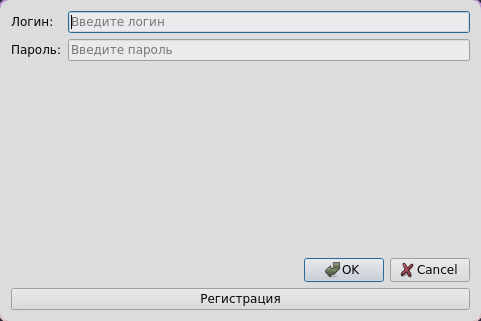
\includegraphics[width=0.6\textwidth]{pics/login.png}
  \caption*{Рисунок 1 - Окно входа в систему}
\end{figure}

\begin{figure}[H]
  \centering
  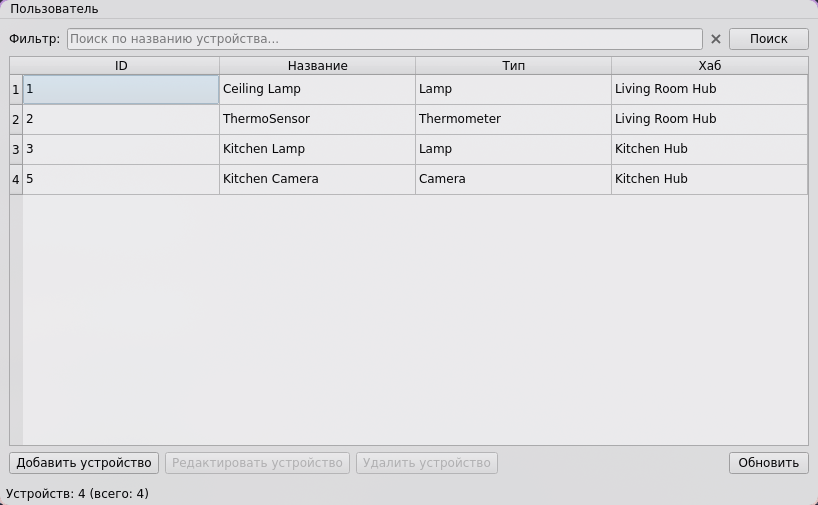
\includegraphics[width=0.8\textwidth]{pics/main_window.png}
  \caption*{Рисунок 2 - Главное окно приложения}
\end{figure}

\begin{figure}[H]
  \centering
  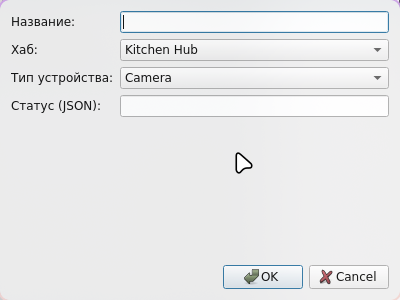
\includegraphics[width=0.6\textwidth]{pics/device_dialog.png}
  \caption*{Рисунок 3 - Диалог добавления устройства}
\end{figure}

\begin{figure}[H]
  \centering
  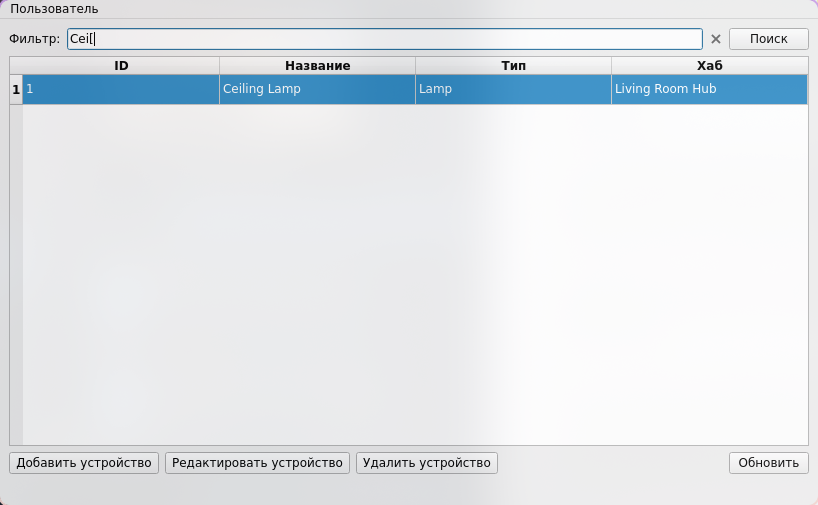
\includegraphics[width=0.95\textwidth]{pics/search_functionality.png}
  \caption*{Рисунок 4 - Функционал ручного поиска}
\end{figure}

\section*{Вывод}

В ходе выполнения лабораторной работы №4 было освоено связывание приложения на C++ с Qt6 с базой данных под управлением PostgreSQL. Разработано приложение с графическим интерфейсом, полностью соответствующее требованиям методических указаний.

\newpage

\section*{Приложение А1. Исходный код main.cpp}
\inputminted{cpp}{code/src/main.cpp}

\section*{Приложение А2. Исходный код database.h}
\inputminted{cpp}{code/src/database.h}

\section*{Приложение А3. Исходный код database.cpp}
\inputminted{cpp}{code/src/database.cpp}

\section*{Приложение А4. Исходный код mainwindow.h}
\inputminted{cpp}{code/src/mainwindow.h}

\section*{Приложение А5. Исходный код mainwindow.cpp}
\inputminted{cpp}{code/src/mainwindow.cpp}

\section*{Приложение А6. Исходный код dialogs.h}
\inputminted{cpp}{code/src/dialogs.h}

\section*{Приложение А7. Исходный код dialogs.cpp}
\inputminted{cpp}{code/src/dialogs.cpp}

\end{document}
